\pagebreak

\chapter{Serial Communication Between the CPU and the FPGA}\label{ch:serialcpu}

    FPGA demonstration boards such as the Gadget Factory Papilio provide a serial
    interface to the FPGA for loading the configuration into the FPGA. These
    interfaces also provide serial communication between the host CPU and the
    FPGA. The 3PL library provides an interface which allows FPGA static, value,
    queue and memory mode variables to be written and read from the CPU and the
    FPGA to interrupt the CPU. For FPGA boards that do not have a serial
    interface inexpensive USB to serial adapters are available.
    
    The FPGA code uses procedures uart\_rx() and uart\_tx() in library uarts.3pl.
    
    This interface is very similar to the Zynq/CPU interface described in the
    next chapter (\autorefph{ch:zynqcpu}). Much of the code is common to
    both. The DMA interface is of course missing here however it is intended
    to add a pseudo-DMA interface.
    
    The CPU to FPGA interfaces are described in \autorefph{chap:lmuartcpulib}.
    
    The board file papilio\_one\_500.3pl for example includes module
    xilinx/uart\_cpu.3pl which includes source xilinx/cpu.3pl and uarts.3pl.
    Trailer procedure create\_bus\_interfaces() in xilinx/uart\_cpu.3pl creates the
    bus interface logic following completion of the main code. 
        
    The board header, e.g. board/gadget\_factory/papilio\_one\_500.3pl,
    will have defined a directive to specify the serial link baud rate,
    directive("comms\_baud\_rate", 115200);.
    
    The following source code, prog.3pl, is an example of a simple 3PL program
    using CPU interfaces -
    
    \begin{lstlisting}[gobble=4, language=threepl]
        module "boards/gadget_factory/papilio_one_500.3pl"
        
        class(cpu, cpu_api());

        static(a, "int:25");
        static(b, "int:18");

        cpu.write(a <- "A");
        cpu.write(b <- "B");

        static(p, "int:48");

        p <- a * b;

        cpu.read(p, "P");

        cpu.receive_event(p == 1, "INT");   // interrupt when p == 1
    \end{lstlisting}
    
    This example has two static mode integer variables, {\bf a} and {\bf b}, that
    can be written to by the CPU. The product is written on every clock cycle to
    static mode integer variable {\bf p}, which can be read by the CPU.
    When {\bf p} is assigned 1 a CPU interrupt is generated
    
    The papilio header file includes module xilinx/uart\_cpu.3pl which in
    turn includes xilinx/cpu.3pl.
    
    The strings "A", "B" and "P" are names with which to refer to the interfaces
    in CPU interface code.
    
    When the program is compiled and executed by 3pl the file (see
    \autorefph{chap:run3pl}) file {\bf prog.info} (amongst others) will be produced.
    
    \begin{verbatim}
        {
            "version": {
                "major": 1,
                "minor": 0
            },
            "directives": {
                "ALU": "false",
                "FIFO": "false",
                "OS": "mac os x",
                "QUEUEREG": "false",
                "arch": "x86_64",
                "comms_baud_rate": "53475",
                "compileOnly": "false",
                "compilerMakeDate": "2022-08-24 14:24:48 +1000",
                "continuous": "false",
                "currentDirectory": "/Users/dun202/src/mine/3PL/test/11.6.0/manual_example_serial",
                "date": "2022-09-23 16:02:55 +1000",
                "designName": "prog",
                "family": "XC3S",
                "filePath": "false",
                "forceExec": "true",
                "gatesNotLuts": "false",
                "intTruncWarning": "false",
                "intermediateOnly": "false",
                "listNets": "true",
                "listTDEs": "true",
                "listTDEsSel": "0",
                "locations": "false",
                "netFile": "/Users/dun202/src/mine/3PL/test/11.6.0/manual_example_serial/prog.net",
                "netlistDisplay": "false",
                "netlistFile": "/Users/dun202/src/mine/3PL/test/11.6.0/manual_example_serial/prog.edn",
                "optimiseConnect": "true",
                "outputDirectory": "/Users/dun202/src/mine/3PL/test/11.6.0/manual_example_serial/",
                "parentDirectory": "/Users/dun202/src/mine/3PL/test/11.6.0/manual_example_serial/",
                "part": "xc3s400aft256-4",
                "postProcessTool": "ise",
                "reportFile": "/Users/dun202/src/mine/3PL/test/11.6.0/manual_example_serial/prog.rpt",
                "rptToFile": "true",
                "sigList": "false",
                "skipPostProc": "true",
                "sourceFile": "prog.3pl",
                "srlAddrWidth": "4",
                "tlimit": "504",
                "uart_cpu": "true",
                "unassOut": "fatal",
                "version": "11.7.0M (devel svn 10083:10129M, dun202)"
            },
            "spaces": {
                "reg": {
                    "bus": "serial",
                    "read_addr_bits": 6,
                    "write_addr_bits": 6,
                    "interfaces": {
                        "infoword": {
                            "interface": "read_value",
                            "write": false,
                            "data_addr": 1,
                            "data_bits": 32,
                            "data_type": {
                                    "type": "uint",
                                    "bits": 32
                            }
                        },
                        "inforeset": {
                            "interface": "write_static",
                            "write": true,
                            "data_addr": 1,
                            "data_bits": 0
                        },
                        "A": {
                            "interface": "write_static",
                            "write": true,
                            "data_addr": 2,
                            "data_bits": 25,
                            "data_type": {
                                    "type": "int",
                                    "bits": 25
                            }
                        },
                        "B": {
                            "interface": "write_static",
                            "write": true,
                            "data_addr": 3,
                            "data_bits": 18,
                            "data_type": {
                                    "type": "int",
                                    "bits": 18
                            }
                        },
                        "P": {
                            "interface": "read_value",
                            "write": false,
                            "data_addr": 2,
                            "data_bits": 48,
                            "data_type": {
                                    "type": "int",
                                    "bits": 48
                            }
                        }
                    }
                }
            },
            "events": {
                "INT": {
                    "intr": 0
                }
            }
        }

    \end{verbatim}
    This file contains a description of the CPU bus interfaces including data
    width, data type and allocated bus address.
    
    A list of the interface functions is written to the report file.
    
    The design.info data may also be stored in block RAM (rmemory) for
    access by CPU code. This is enabled by default but may be avoided via a
    directive, i.e. {\bf directive("excludeinfo", true);}, which can be executed
    at any time during 3PL immediate execution. The embedded .info is only
    useful for Python application code as there is no easy wasy to incorporate
    the interface description into an executing C program.
    
    The compression is done by
    calling inbuilt function {\bf deflate()} \autorefph{sec:ifdeflate}. The
    readback is initialised by writing to address 1 and 32-bit packed .info data
    is then read by successive 32-bit reads from address 1. The first read
    returns a 32 bit CRC-32 checksum for the remainder of the block,\. The
    second read returns the uncompressed data size in bytes and the third read
    returns the compressed data size in bytes. Reads beyond the data length will
    return zeros.
    
    The data block size depends on the size of the compressed .info data and
    varies from a minimum of 1024 32 bit words (1 RAM block) to 32,768 words (32
    RAM blocks).

    
    
    

    \section{C interface}
    
        The python script info2c (in directory tools/serial/info2c)
        reads the .info file and produces a C .h include file, e.g.
        \begin{lstlisting}[gobble=4, language=C]
            info2c prog
        \end{lstlisting}
        reads file {\bf prog.info} and produces {\bf prog\_fpga.h}.
        This file provides a wrapper for each FPGA interface. These
        in turn call functions in {\bf fpga.c}. The application must also
        directly call {\bf fpga\_open()} and {\bf fpga\_close()} in fpga.c.
        
        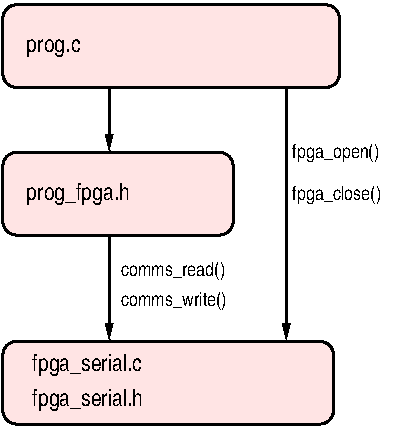
\includegraphics{c_serial}
        
        For details see (\autorefph{ch:tools_c_serial}).
        
        For the .info file listed previously the created include file
        {\bf prog\_fpga.h} contains -

        \begin{lstlisting}[gobble=4, language=C]
            // interface "P" in space "reg" 
            typedef int64_t fpga_P_t;
            const unsigned fpga_P_addr = 2;
            static fpga_P_t
            fpga_P_read() {
                fpga_P_t v;
                comms_read(0, fpga_P_addr, 0, 6, 1, 2, (char *)&v);
                if ((v & 0x800000000000) != 0)
                    v |= 0xffff000000000000;
                return(v);
            }

            // interface "B" in space "reg" 
            typedef int32_t fpga_B_t;
            const unsigned fpga_B_addr = 3;
            static void
            fpga_B_write(fpga_B_t val) {
                comms_write(0, fpga_B_addr, 0, 3, (char *)&val);
            }

            // interface "A" in space "reg" 
            typedef int32_t fpga_A_t;
            const unsigned fpga_A_addr = 2;
            static void
            fpga_A_write(fpga_A_t val) {
                comms_write(0, fpga_A_addr, 0, 4, (char *)&val);
            }

            // event "INT"
            void
            fpga_INT_wait() {
                sem_wait(sem[0]);
            }

            const unsigned fpga_interrupts = 1;
        \end{lstlisting}
        Note that for each interface function the string "fpga\_" is prepended
        to the function identifier.

        At the moment reads and writes of single variables will defines types
        {\bf int8\_t} or {\bf uint8\_t} up to {\bf int\_64\_t} or {\bf uint64\_t}
        for data widths 8, 16, 32 or 64. A struct up to 64 bits in size will be
        mapped to a bit field.
    
        The following C program includes the above file -        

        \begin{lstlisting}[gobble=4, language=C]
            #include <stdio.h>
            #include "cpu_serial.h"

            void*       INT_handler ();

            #include    "prog_fpga.h"

            int
            main (
                int     argc,
                char**  argv
            ) {    
                pthread_t   INT_thread;
                int         pri_min = 1;

                // Establish the CPU interface.
                fpga_open("/dev/tty.usbmodem14201");

                // Start a thread for the interrupt
                INT_thread  = thread_start(INT_handler,  "INT_handler",  pri_min);

                fpga_A_write(123);
                fpga_B_write(1);
                printf("read %lld (should be 123)\n", fpga_P_read());
                fpga_A_write(1);   // will generate an interrupt
                sleep(1);          // wait for the interrupt

                // Close the interrupt thread.
                pthread_cancel(INT_thread);


                // Close the CPU interface.
                fpga_close();

                exit(0);
            }

            void*
            INT_handler () {
                for(;;) {
                    fpga_INT_wait();
                    printf("interrupt INT\n");
                }
            }

        \end{lstlisting}

        The CPU code uses library {\bf cpu\_serial.c} (see appendix
        \ref{ch:cpu_serial}) and hence the application program must be
        linked to cpu\_serial.o.

        Procedure findserialdev() is called to find the file path for the serial
        device to which the FPGA board is connected. In this case the code is
        for Apple OSX and device names will be different in Linux or Unix.

        fpga\_open() opens the serial device, starts
        a thread to handle the communications and establlishes any semaphores
        required for interrupts. Writes to the FPGA do not supply any
        acknowledgement. Data returned from the FPGA included requested reads
        and asynchronous 'interrupts'. Details of the interface are described in
        \autorefph{chap:lmxilcpulib}.

        fpga\_close() terminates the thread, removes any semaphores and
        closes the serial port.

        Bus interfaces are used by calling the appropriate subroutines defined
        in prog\_fpga.h, in this case {\bf fpga\_A\_write()},  {\bf fpga\_B\_write()}
        and {\bf fpga\_P\_read()}, the bus addresses having been subsumed into
        the subroutine definitions.
    



    \section{Python interface}

        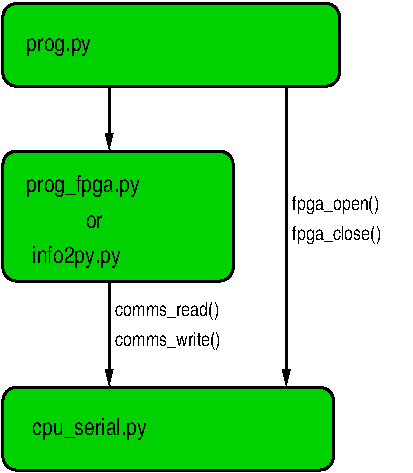
\includegraphics{py_serial}
        
        For details see (\autorefph{ch:tools_python_serial}).
        
        The 3PL module uart\_cpu.3pl will always produce a .info file. A
        compressed version loaded into block RAM in the FPGA configuration will
        also be included by default but can be omitted by creating the directive
        "excludeinfo".
    
        For a Python interface to the FPGA the module {\bf cpu\_serial.py} (in
        directory fpga\_platforms/serial/uart\_cpu must be imported.)
        
        Optionally {\bf info2py.py} (in directory fpga\_platforms/info2py) can
        be imported to convert the .info file to an internal compiled Python3
        module.        If {\bf info2py.py} is imported it either reads the .info
        file (call info\_from\_file(file) or downloads the compressed info data
        in the FPGA (call info\_from\_fpga()) and generates an internal module
        containing functions to access the FPGA register or memory interfaces.

        As an alternative the Python3 script {\bf info2py} can be executed
        to create a Python3 module {\bf prog\_fpga.py} which is then imported
        into the application program. A version of this file
        for the present example is listed below -


        \begin{lstlisting}[gobble=4, language=Python]
            import os
            import math
            import string
            import textwrap
            import argparse
            import json
            import sys
            import time
            sys.path.append(os.environ['HOME'] + '/install/3pl')
            import cpu_serial as fpga_rw

            def B_write(wdata):
                val = wdata 
                if val < 0:
                    wba = val.to_bytes(3, byteorder='little', signed=True)
                else:
                    wba = val.to_bytes(3, byteorder='little')
                fpga_rw.comms_write(0, 3, 0, wba)

            def P_read():
                rba = fpga_rw.comms_read(0, 2, 0, 6)
                val = int.from_bytes(rba, byteorder='little', signed=False)
                fval = val & 0xffffffffffff
                if (fval & 0x800000000000) != 0:
                     fval = -((fval ^ 0xffffffffffff) + 1)
                return(fval)

            def A_write(wdata):
                val = wdata 
                if val < 0:
                    wba = val.to_bytes(4, byteorder='little', signed=True)
                else:
                    wba = val.to_bytes(4, byteorder='little')
                fpga_rw.comms_write(0, 2, 0, wba)

            # event "INT"
            def INT_wait():
                fpga_rw.semaphores[0].acquire()

            def INT_count():
                return(fpga_rw.event_count(0))
        \end{lstlisting}



        cpu\_serial.py provides the code to open the serial interface to the FPGA,
        read and write to the FPGA and generate interrupts if required.

        
        The identifiers of the interface functions are listed in the report file,
        along with the data type. Each function is contained in the CPU\_API class
        {\bf fpga}.
        
        Python source code equivalent to the previous C interface might be -
        \begin{lstlisting}[gobble=4, language=Python]
            import sys
            sys.path.append("/Users/....../install/3pl")
            import info2py
            from cpu_serial import *
            import time
            import signal
            import threading

            fpga_open("/dev/tty.usbmodem14101")

            fpga = info2py.info_from_fpga()         # load info from FPGA

            def INT_handler():
                while True:
                    fpga.INT_wait()
                    print("event INT")

            ev_INT = threading.Thread(target=INT_handler, args=(), daemon=True)
            ev_INT.start()

            a = 123
            b = 1

            fpga.A_write(a)
            fpga.B_write(b)
            print(str(fpga.P_read()) + "\t(should be 123)")
            a = 1
            fpga.A_write(a);    # will generate an interrupt

            time.sleep(1.0)     # wait for the interrupt

            fpga_close()

            os.kill(os.getpid(), signal.SIGTERM)    # use this to kill all threads!
        \end{lstlisting}
        
        In the code above the application program loads the interface information
        from the version embedded in the FPGA in block RAM.
        With the following modification the interface information will be
        loaded from the prog.info file instead.

        
        \begin{lstlisting}[gobble=4, language=Python]
            import sys
            .
            .
            .

            fpga_open("/dev/tty.usbmodem14101")
            
            fpga = info2py.info_from_file("prog")   # load info from prog.info file
            .
            .
            .
        \end{lstlisting}
        
        
        
        Alternatively the following imports a version of the interface function
        definitions created by Python3 script {\bf info2py}.
        
        \begin{lstlisting}[gobble=4, language=Python]
            import sys
            .
            .
            .
            import prog_fpga as fpga    # import interface info from Python3 file

            fpga_open("/dev/tty.usbmodem14101")
            .
            .
            .
            .
        \end{lstlisting}
        
        
        The Python serial interface to the FPGA can read or write variables of
        any type to any degree of nesting, but there is a maximum variable size
        of 1016 bits (the 7-bit byte count in the communication protocol limits
        the data length to 127 bytes). The following type conversions between
        3PL and Python will occur -
         
        \begin{tabular}{| l | l | l |}
        \hline
        FPGA    & Python                \\
        \hline
        log     & logical               \\
        bits    & integer               \\
        uint    & integer               \\
        int     & integer               \\
        ufixed  & IEEE754 64bit float   \\
        fixed   & IEEE754 64bit float   \\
        float   & IEEE754 64bit float   \\
        struct  & dictionary            \\
        array   & list                  \\
        \hline
        \end{tabular}
        
        There are no run-time tests for data integrity, for example overflows.
        
        3PL arbitrary ufixed and fixed integer and fraction sizes are converted
        in or out of IEEE 64 bit floatin point in Python. Similarly 3PL arbitrary
        floating point biased exponent and mantissa sizes are again converted
        in or out of IEEE 64 bit floatin point.
        
        A struct in 3PL is converted in or out of a dictionary in Python, the
        field name being the key.
        
        3PL multi-dimensional arrays are nested lists in Python.
